\newenvironment<>{redblock}[1]{%
  \setbeamercolor{block title}{fg=white,bg=red!75!black}%
  \begin{block}#2{#1}}{\end{block}}

  
%%%%%%%%%%%%%%%%%%%%%%%%%%%%%%%%%%%%%%%%%%%%%%%%%%%%%%%%%%%%%%%%%%%%%%
% Slides
%%%%%%%%%%%%%%%%%%%%%%%%%%%%%%%%%%%%%%%%%%%%%%%%%%%%%%%%%%%%%%%%%%%%%%

\begin{frame}
\titlepage
\end{frame}

\begin{frame}{Sumário}
  \tableofcontents
\end{frame}
\selectlanguage{brazil}
\section{Justificativa}

\begin{frame}{Justificativa}
  \begin{itemize}
   \setlength\itemsep{2em}

   \item Perspectiva acadêmica
   \begin{itemize}
      \item[\checkmark] Poucos trabalhos que comparam protocolos de enlace que solucionam o problema dos nós em silêncio com múltiplos canais
   \end{itemize}
   \item Perspectiva econômica
   \begin{itemize}
      \item[\checkmark] Estudos de casos podem indicar as configurações de maior vazão em redes ad hoc de múltiplos saltos e múltiplos canais
   \end{itemize}
  \end{itemize}
\end{frame}


\section{Fundamentação Teórica}

\begin{frame}{Modelo de Referêcia}
  \begin{columns}
    \column{0.7\textwidth}
     $[5]$ Aplicações utilizadas pelos usuários \\
     $[4]$ Fracionamento e distribuição dos pacotes \\
     $[3]$ Roteamento \\
     $[2]$ Controle de acesso ao canal e detecção de falhas e erros \\
     $[1]$ Transmissão de bits: \\ 
     \hspace{35pt} De 0.0 à 0.8 Volts - bit 0 \\
     \hspace{35pt} De 2.0 à 5.0 Volts - bit 1
    \column{0.3\textwidth}
    \begin{figure}
      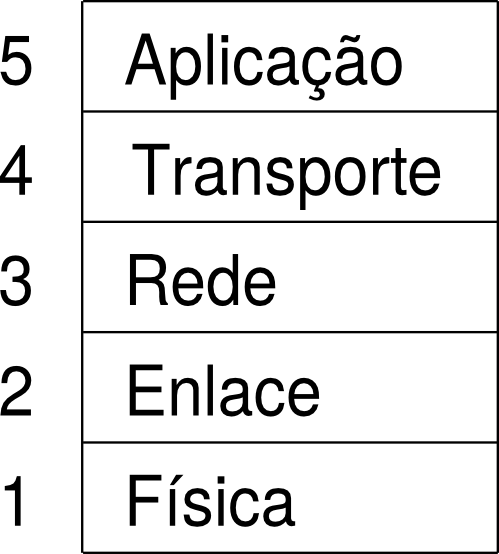
\includegraphics[width=\textwidth]{camadas}
      \caption{Modelo de referência usado por Tanenbaum [1].}
      \label{fig:camadas}
    \end{figure}
  \end{columns}
\end{frame}

\begin{frame}{Redes ad hoc}
 \begin{columns}
    \column{0.4\textwidth}
    \begin{itemize}
    \item Não possui ponto de acesso
    \item Aparelhos (nó) são todos roteadores e possuem alcances diferentes
    \item É auto-configurável
    \item Ultiliza \textit{handshake} para realizar a comunicação. Exemplo: RTS/CTS
    \end{itemize}

    \column{0.6\textwidth}
    \begin{figure}
      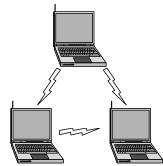
\includegraphics[width=0.5\textwidth]{FiguraIntro}
      \caption{Comunicação em uma rede ad hoc [1].}
      \label{fig:FiguraIntro}
    \end{figure}
  \end{columns}
\end{frame}


\begin{frame}{Redes ad hoc - Exemplos}
   \begin{columns}
    \column{0.4\textwidth}
    \begin{figure}
      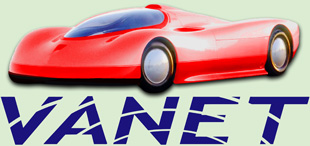
\includegraphics[width=0.8\textwidth]{vanet}
      \caption{Vehicular Ad hoc Networks (VANETs) [2].}
      \label{fig:vanet}
    \end{figure}

    \column{0.6\textwidth}
    \begin{figure}
      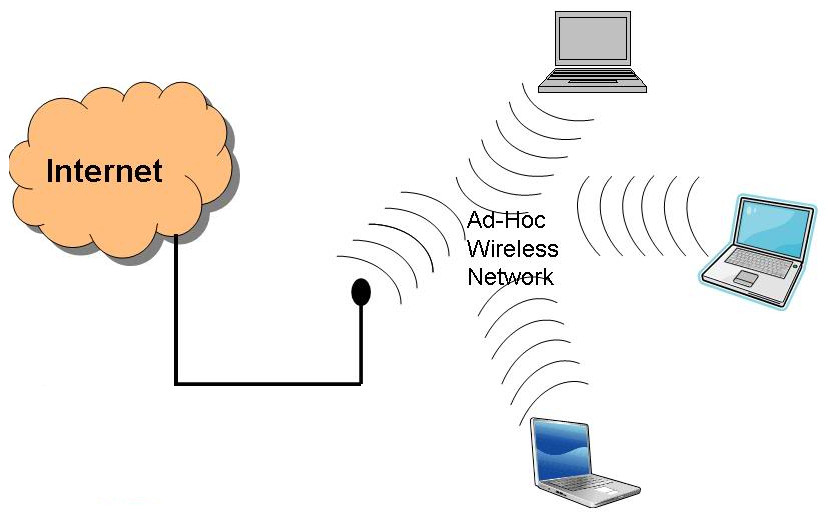
\includegraphics[width=0.9\textwidth]{imanet}
      \caption{Internet based mobile ad hoc networks (iMANETs), adaptado de [3].}
      \label{fig:imanet}
    \end{figure}
  \end{columns}

\end{frame}


\begin{frame}{Redes de múltiplos saltos}
 \begin{columns}
    \column{0.4\textwidth}
    \begin{itemize}
    \item Maior flexibilidade
    \item Maior \textit{delay}
    \item Caminho indireto até o destino
    \item Rota é tabelada dinamicamente
    \item A maneira como a tabela é criada depende do protocolo da Camada de Rede
    \end{itemize}

    \column{0.6\textwidth}
    \begin{figure}
    \setlength\itemsep{2em}
      \includegraphics[width=\textwidth]{multiSaltos}
      \caption{O pacote deve passar por um ou mais nós até chegar ao destino [4].}
      \label{fig:multiSaltos}
    \end{figure}
  \end{columns}
\end{frame}

\begin{frame}{Redes de múltiplos canais}
 \begin{columns}
    \column{0.4\textwidth}
    \begin{itemize}
    \item Maior vazão
    \item Previne colisões
    \item Cada canal é uma faixa de frequência diferente
    \item A maneira como os nós são distribuídos nos canais depende do protocolo da Camada de Enlace
    \end{itemize}

    \column{0.6\textwidth}
    \begin{figure}
      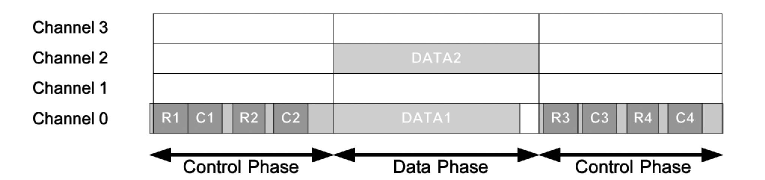
\includegraphics[width=\textwidth]{canal_MMAC}
      \caption{Ilustração do protocolo MMAC [5].}
      \label{fig:canal}
    \end{figure}
    
    \begin{figure}
      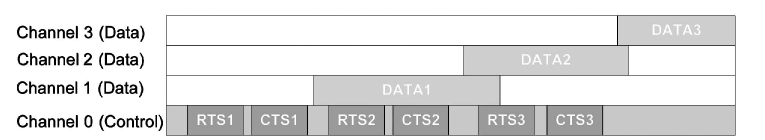
\includegraphics[width=\textwidth]{canal_DCA-PC}
      \caption{Ilustração do protocolo DCA-PC [5].}
      \label{fig:canal}
    \end{figure}
  \end{columns}
\end{frame}



\section{Problema e Hipóteses}

\begin{frame}{O Nó em Silêncio}
 
 \begin{figure}
      \includegraphics[width=0.7\textwidth]{SilencedNode}
      \caption{Cenário da situação-problema, adaptado de [4]}
      \label{fig:SilencedNode}
    \end{figure}
\end{frame}

\begin{frame}{O Nó em Silêncio}
  \begin{redblock}{Problema}
   Comparar protocolos da camada de enlace que amenizam ou solucionam o problema do Nó em Silêncio em uma rede ad hoc sem fio 
   mantendo alta vazão e baixo \textit{delay}.
  \end{redblock}
  \begin{block}{Hipótese}
   Uma rede que ad hoc realista, ou seja, que forneça suporte à múltiplos saltos pode obter alto desempenho com a
   utilização de protocolos que permitam múltiplos canais.
  \end{block}
\end{frame}



\section{Objetivos}

\begin{frame}{}

  \begin{block}{Objetivo Geral}
  Verificar as semelhanças e diferenças entre protocolos da Camada de Enlace que possuam os mais altos 
  desempenhos enquanto resolvem ou amenizam o problema do Nó em Silêncio.
  \end{block}
  \begin{block}{Objetivos Específicos}
    \begin{itemize}
    \item Encontrar diferentes soluções para o problema do Nó em Silêncio
    \item Implementar tais soluções com no mínimo 2 protocolos de enlace diferentes
    \item A partir dos resultados esperados, como tempo de execução, número de eventos realizados e vazão, fazer uma tabela comparando os protocolos de enlace
    \end{itemize}
  \end{block}
\end{frame}

\section{Metodologia}

\begin{frame}{Sistematização}
  \begin{block}{Revisão bibliográfica}
    Selecão dos protocolos a serem utilizados nas simulações
  \end{block}
  \begin{block}{Familiaridade com ambiente de simulação OMNet++}
    Aprendizado da linguagem de programação NED
  \end{block}
  \begin{block}{Implementação}
    Realização de vários estudos de casos modificando alguns parâmetros em cada protocolo de enlace
  \end{block}
  \begin{block}{Interpretação dos resultado}
    Avaliação e comparação das eficiências de cada caso
  \end{block}
\end{frame}


\begin{frame}{Cronograma}
  \begin{table}[h!]
  \centering
  %\captionsetup{labelsep=space,justification=justified,singlelinecheck=off}
  \caption{Cronograma}
    \begin{tabular}{|l|c|c|c|c|c|c|c|c|c|}
    \hline
    \multirow{2}{*}{Atividades}  & \multicolumn{7}{c|}{2015} \\ \cline{2-8}
    & Jun & Jul & Ago & Set & Out & Nov & Dez \\ \hline
    \begin{tabular}[x]{@{}c@{}}Revisão\\bibliográfica\end{tabular} & X & X & X &  &  &  &  \\ \hline
    \begin{tabular}[x]{@{}c@{}}Familiaridade\\com OMNet++\end{tabular}  & X & X & X & X &  &  &  \\ \hline
    Implementação  &  &  & X & X & X &  &  \\ \hline
    \begin{tabular}[x]{@{}c@{}}Interpretação\\dos resultado\end{tabular}  &  &  &  & X & X & X & X \\ \hline 
    Defesa  &  &  &  &  &  &  & X \\ \hline
    \end{tabular}
  \end{table}
\end{frame}

\section{Referências}

\begin{frame}
  \frametitle{Referências}
  \begin{itemize}
    \item \footnotesize Sunil Kumar, Vineet S. Raghavan, and Jing Deng. Medium access control protocols for ad hoc wireless networks: A survey. Ad Hoc Netw., 4(3):326–358, Maio 2006.
    \item \footnotesize Shih-Lin Wu, Yu chee Tseng, Chih-Yu Lin, and Jang-Ping Sheu. A multi-channel mac protocol with power control for multi-hop mobile ad hoc networks. The Computer Journal, 45:101–110, 2002.
    \item \footnotesize Hoi-Sheung Wilson So, Jean C. Walrand, and Jeonghoon Mo. Mcmac: A parallel rendezvous multi-channel mac protocol. In WCNC, pages 334–339. IEEE, 2007.
    \item \footnotesize Jeonghoon Mo, Hoi-Sheung So, and Jean Walrand. Comparison of multichannel mac protocols. IEEE Transactions on Mobile Computing, Janeiro 2008.
  \end{itemize}
\end{frame}

\begin{frame}
  \frametitle{Referências das figuras}
  \begin{enumerate}
    \item \footnotesize Andrew S. Tanenbaum and David J. Wetherall. Computer Networks. Prentice Hall, 5th edition, 2011.
    \item \footnotesize The Fourth ACM International Workshop on Vehicular Ad Hoc Networks (VANET 2007), http://www.sigmobile.org/workshops/vanet2007/, visitado em 2015-06-20
    \item \footnotesize Ad-hoc NETwork, https://sites.google.com/a/ochin.mygbiz.com/my-scientific-work/my-academic-work/openvanet, visitado em 2015-06-20
    \item \footnotesize S. Basagni, M. Conti, S. Giordano, and I. Stojmenovic. IEEE 802.11 AD HOC Networks: Protocols, Performance, and Open Issues. Wiley-IEEE Press, Pisa, Itália, Outubro 2004
    \item \footnotesize Jeonghoon Mo, Hoi-Sheung So, and Jean Walrand. Comparison of multichannel mac protocols. IEEE Transactions on Mobile Computing, Janeiro 2008.
  \end{enumerate}
\end{frame}

\appendix

\begin{frame}
  \frametitle{Obrigada pela atenção!}
  \begin{center}
    {\Huge Obrigada!}
  \end{center}
\end{frame}

\begin{frame}
  \frametitle{Perguntas e Respostas}
  \begin{center}
    {\Huge Perguntas?}
  \end{center}
\end{frame}